\paragraph{В третьей} главе ставиться задача разработки алгоритма оценки информационных параметров CDMA-сигнала на основе алгоритма Delay and Multiply Approach,
предлагаемого усовершенствованного итеративного алгоритма вычисления АКФ и АР модели второго порядка.

В работе предлагается комплексировать результаты работы алгоритма Delay and Multiply Approach и, предложенных
в данной работе, усовершенствованного итеративного алгоритма уточнения АКФ гармонического
сигнала и подхода для оценки частоты CDMA-сигнала при помощи АР-модели.

При наличии нескольких источников CDMA-сигнала в смеси присутствует помеха в полосе сигнала.
После оцифровки и повторного модулирования входной смеси (\ref{eq:cdma_eq}) с ПСП в данном случае получается:
\begin{equation}
	\label{eq:cdma_strip_eq}
	x_k(m) = A_k \cos{(\tilde{\omega}_{k}m + \phi_k(m))} + n_k(m) + i(m)
\end{equation}
где ${m}$ - индекс соответствующий времени, ${\tilde{\omega}_k}$ - нормированная частота, соответствующая ${\omega_k}$, ${n_k}(m)$ - шум ${n(t)}$, умноженный на ПСП,
${i(m)}$ - интерференционная помеха.

Интерференционная составляющая ${i(m)}$ представляет собой сигнал от других источников, модулированный ПСП искомого источника сигнала:
\begin{equation}
	\label{eq:cdma_interference}
	i(m) = g_k(t) \sum\limits_{i=1, i \ne k}^{N}A_i g_i(t)\cos{(\omega_{i}m + \phi_i(m))}
\end{equation}

Схематично приемник изображен на рисунке \ref{pic:ar_dma_scheme}.
\begin{figure}[h]
\center\scalebox{1}{\includegraphics[width=1\linewidth]{dma_quadruple_lpc.eps}}
	\caption{Алгоритм обнаружения и оценки параметров ШПС в условиях интерференции (DMA + уточненный АР)}
	\label{pic:ar_dma_scheme}
\end{figure}

Выходом алгоритма Delay and Multiply Approach является оценка фазы ПСП. Повторно модулируя входную смесь с ПСП,
можно восстановить гармонический сигнал при условии правильной оценки фазы ПСП. Для оценки частоты данного сигнала применяется
АР-метод. Но для оценки АР-методом, требуется точная оценка АКФ, которую можно получить
с помощью усовершенствованного итеративного алгоритма вычисления АКФ.

{\underline{Предложенный алгоритм можно описать следующим набором шагов:}}
\begin{itemize}
\item[Шаг 1.] Входной сигнал ${x(m)}$ умножается на задержанную копию ${x(m-\tau)}$. Так же
	на данном шаге можно производить когерентное накопление результата, для
	увеличения ОСШ.

	\begin{center}
	\begin{equation}
		%\label{}
		x_{new}(m) = \frac{g_{new}(k)}{2} \left(\cos (2\pi f \tau) - \cos \left[2 \pi f (2m - \tau)\right]\right)
	\end{equation}
	\end{center}

\item[Шаг 2.] Полученный сигнал ${x_{new}(m)}$ фильтруется ФНЧ для отсечения высокочастотной компоненты.
\item[Шаг 3.] Генерируется локальная ПСП ${C(m)}$ и умножается на задержанную копию ${g(m-\tau)}$.

	\begin{center}
	\begin{equation}
		%\label{}
		g_{new}(m) = g(m)g(m-\tau)
	\end{equation}
	\end{center}

\item[Шаг 4.] Отфильтрованный сигнал ${x_{filt}(m)}$ коррелируется с новой ПСП ${g_{new}(m)}$
	с использованием БПФ. Выход коррелятора сравнивается с заранее определенным порогом.

	\begin{center}
	\begin{equation}
		%\label{}
		x_{filt}(m) = \frac{g_{new}(m)}{2} \cos (2\pi f \tau)
	\end{equation}
	\end{center}

	\subitem{\underline{Если}}  значение оказалось больше порогового {\underline{то}},
		принимается решение о наличии сигнала. Полученное значение фазы ПСП  - ${k}$ запоминается.
		Перейти на шаг 5.
	\subitem{\underline{Иначе}} 
		Выбирается ${N}$ максимальных значений и запоминаются их фазы ПСП.
\item[Шаг 5.] Входная смесь ${x(m)}$ модулируется ПСП ${g(m-k)}$, где ${k}$ - это оценка фазы ПСП. В результате получаем гармонический
	сигнал ${x_{cos}(m)}$ с неизвестной частотой.
\item[Шаг 6.] Для увеличения ОСШ сигнала ${x_{cos}(m)}$ вычисляется значение уточненное значение АКФ
	по усовершенствованному итеративному алгоритму получения АКФ.
\item[Шаг 7.] Определяются коэффициенты АР-модели ${\hat{a_1}, \hat{a_2}}$.
	Вычисляется резонансная частота ${\omega_1}$ и определяется квадрат модуля частотного отклика АР-модели для этой частоты. 
\item[Шаг 8.]
	Сравнение квадрата модуля с порогом.
        \subitem{\underline{Если}}  значение оказалось больше порогового {\underline{то}} 
                принимается решение о наличии сигнала, а в качестве оценки
                частоты принимается значение ${\omega_1}$ соответствующее выбранной фазе ПСП. 
        \subitem{\underline{Иначе}} 
		\subsubitem\underline{Если} остались непроверенные фазы ПСП - переход на шаг 5.
		\subsubitem\underline{Иначе} сигнал не обнаружен.
\end{itemize}

График вероятности оценки частоты в допустимом диапазоне входной расстройки ФАПЧ для одной, двух и трех итераций уточнения АКФ представлен на рисунке
\ref{pic:ar_dma_probability}. Моделирование проводилось с аддитивным шумом, заданным в полосе от 0 Гц до
половины частоты дискретизации для одного, двух и трех шагов уточнения АКФ. В данной имитационной модели значение частоты дискретизации равно 16.368 МГц.
\begin{figure}[h]
\center\scalebox{1}{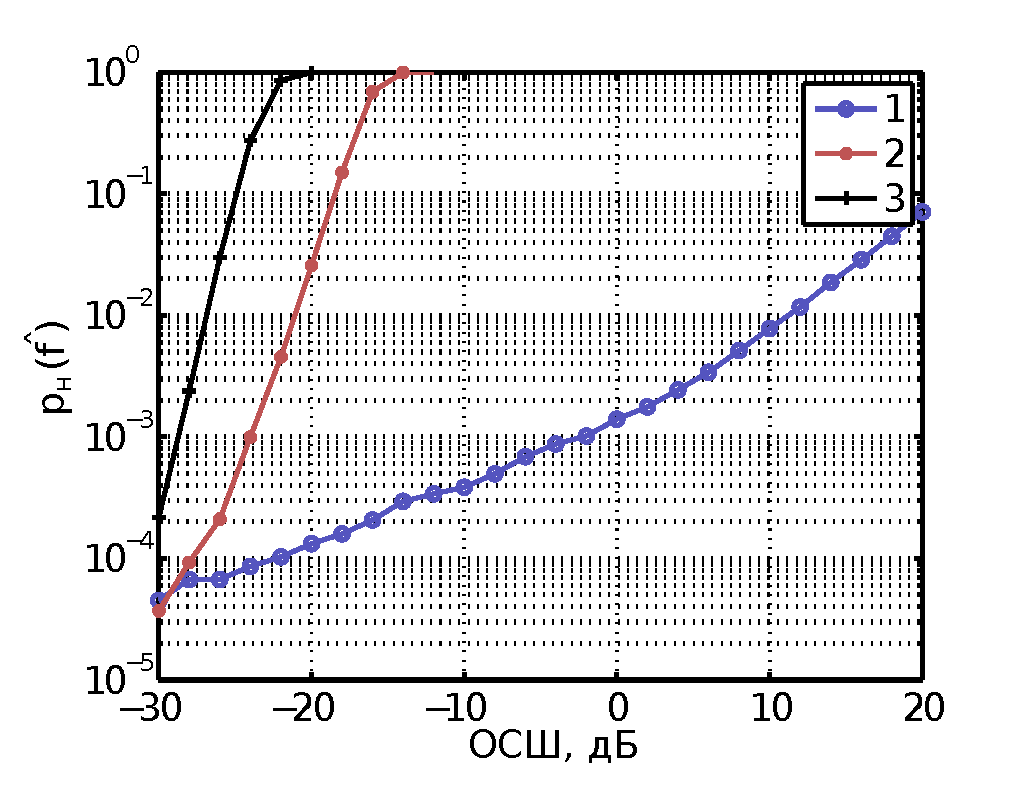
\includegraphics[width=1\linewidth]{ar_dma_probability.eps}}
	\caption{Вероятность оценки частоты удовлетворяющей допустимой входной расстройке. 1 - одна итерация вычисления АКФ, 2 - две итерация вычисления АКФ, 3 - три итерации вычисления АКФ}
	\label{pic:ar_dma_probability}
\end{figure}

Так же в работе проводилось сравнение качества оценки частоты. График СКО ошибки при оценке частоты в зависимости
от ОСШ представлен на рисунке \ref{pic:crlb_vs_snr}. Для сравнения так же взята граница Крамера-Рао (КР).
\begin{figure}[h]
\center\scalebox{1}{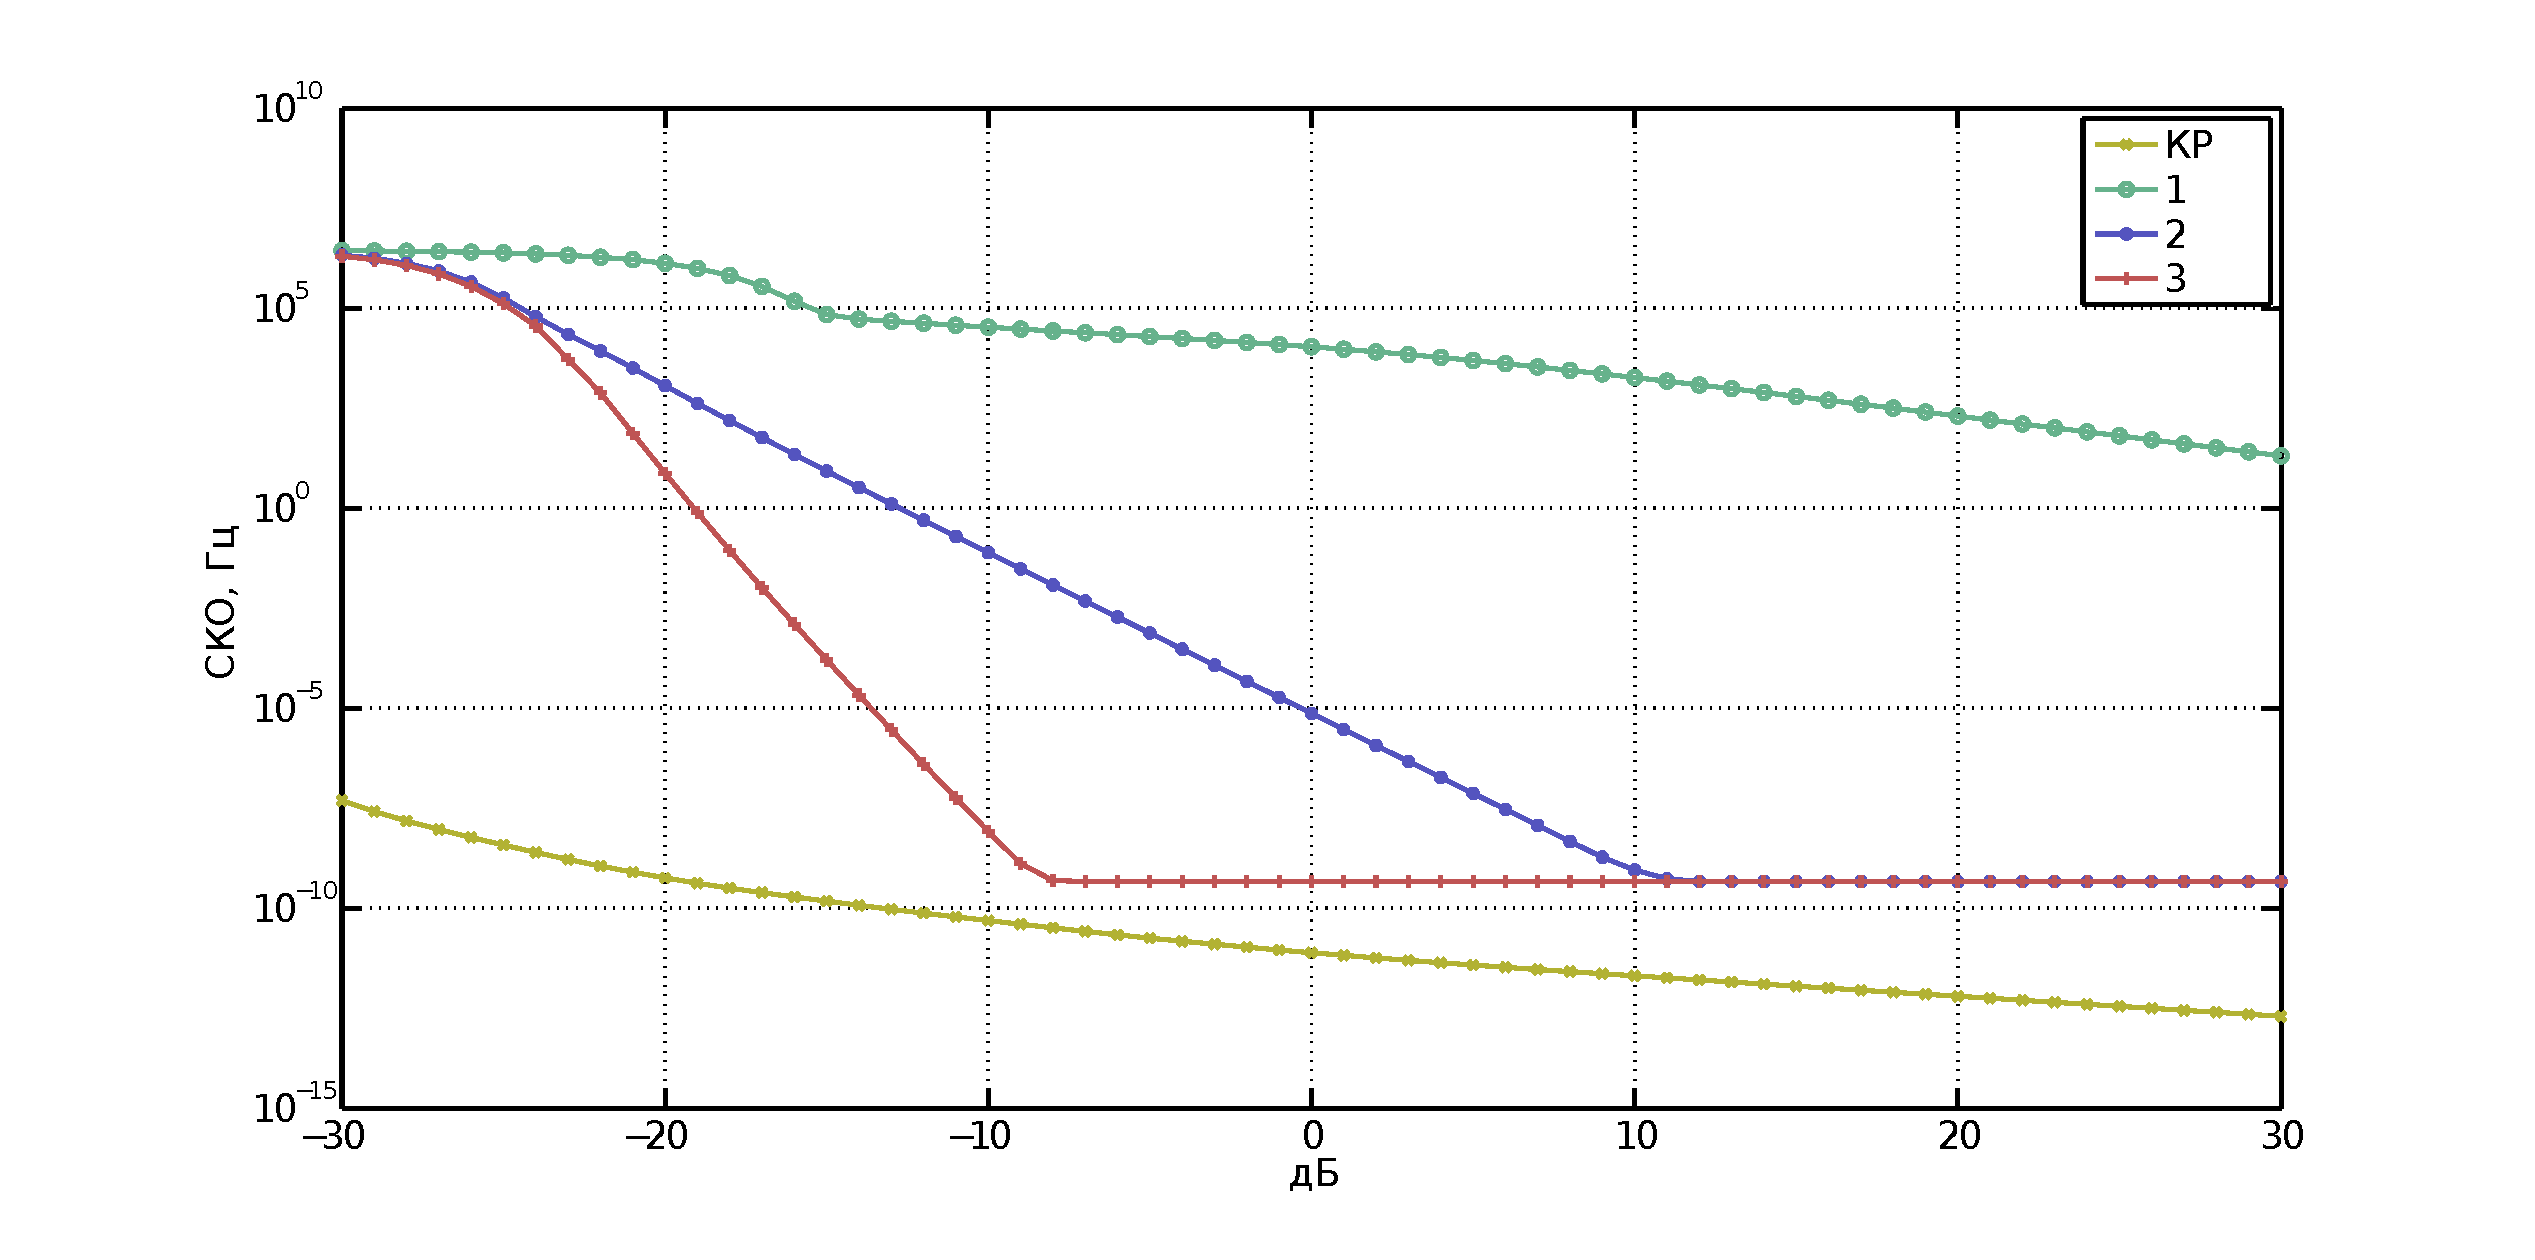
\includegraphics[width=1\linewidth]{crlb_vs_snr.eps}}
	\caption{СКО ошибки оценки частоты и граница Крамера-Рао в задаче оценки частоты гармонического сигнала.}
	\label{pic:crlb_vs_snr}
\end{figure}

Единственным ограничением является наличие только одной гармонической компоненты в принимаемом сигнале.

Общее количество умножений, необходимых для оценки информационных параметров CDMA-сигнала от одного источника предлагаемым
алгоритмом (количество итераций в алгоритме уточнения АКФ равно 3): ${OP_{DMA\_ACF\_AR} = 16NlogN + 11N + 51}$.

Количество итераций требуемых для оценки частоты одного источника параллельным коррелятором:
${OP_{corr} = 48NlogN + 65N}$. Для оценки частоты берется входная последовательность равная 1 мс, что позволяет
получить точность 1 кГц, шаг одной итерации выбран в 1 кГц.

Предлагаемый подход существенно выигрывает по вычислительным затратам в сравнении с параллельным коррелятором при
меньших вычислительных затратах.
